
\section{Неделя III}

\subsection*{№1 (1.3.4)}


Найдём решение уравнения
\begin{equation*}
    \int_{0}^{t} K(t-s) f(s) \d s = \varphi(t),
    \hspace{10 mm} 
    K(t) = t,
    \hspace{5 mm}
    \varphi(t) = \sin (t).
\end{equation*}
Решение может быть найдено, как
\begin{equation*}
    \tilde{f}(p) = \frac{\tilde{\varphi}(p)}{\tilde{K}(p)},
    \hspace{10 mm} 
    f(t) = 
    \int_{c-i \infty}^{c+i \infty} \frac{\d p}{2 \pi i} \exp(pt) \tilde{f}(p).
\end{equation*}
Для начала найдём, что
\begin{equation*}
    \tilde{\varphi}(p) = \int_{0}^{\infty} e^{- p t} \frac{e^{i t} - e^{- i t}}{2 i} \d t = 
    \frac{-1}{2i}\left(
        \frac{1}{i-p} + \frac{1}{i+p}
    \right) = \frac{1}{1+p^2}.
\end{equation*}
А также изображение для возмущения
\begin{equation*}
    \tilde{K}(p) = -\left(
        \int_{0}^{\infty} \exp\left(-p t\right) 
    \right)'_p = 
    \left(
        \frac{1}{p} e^{- pt} \big|_0^{\infty}
    \right)'_p = \frac{1}{p^2}.
\end{equation*}
Заметим, что $\lim_{p \to \infty} \tilde{f}(p) = 1$, тогда
\begin{equation*}
    f(t) = \delta(t) + \int_{c-i \infty}^{c+i \infty} \frac{d p}{2 \pi i} e^{pt} \left(
        \frac{p^2}{1+p^2}-1
    \right) = 
    \delta(t) - \int_{c-i \infty}^{c+i \infty} \frac{d p}{2 \pi i} e^{pt} \left(
        \frac{1}{1+p^2}
    \right) = \delta(t) - \sin (t),
\end{equation*}
где воспользовались уже известным значением изображения синуса. 

Для галочки можем посчитать оригинал напрямую. Тогда заметим, что полюса находятся в $p = \pm i$, соответственно возьмём $c = 1$ и сделаем замену $p = 1 + i \omega$, тогда придём к интегралу
\begin{equation*}
    - e^{t} \int_{-\infty}^{+\infty} \frac{\d \omega}{2\pi} \frac{e^{i \omega t}}{[\omega - (1+i)][\omega-(-1+i)]}
    = - e^{t} \left(
        \frac{1}{2} i e^{(-1-i) t}-\frac{1}{2} i e^{(-1+i) t}
    \right) = \sin (t),
\end{equation*}
в общем, всё сходится.


\subsection*{№2 (1.4.2)}


Найдём функцию Грина
\begin{equation*}
    G(t,\,  s) = \theta(t-s) \exp\left(
        - \int_{s}^{t} \gamma(\tau) \d \tau
    \right),
\end{equation*}
для $\gamma(t) = a/t$, где $a = \const$.  Нетрудно найти, что
\begin{equation*}
    G(t, s) = \theta(t-s) \exp\left(
        - a \ln \frac{t}{s}
    \right) = \theta(t-s) \left(\frac{s}{t}\right)^a.
\end{equation*}




\subsection*{№3 (1.5.1)}


\textbf{Общее замечание}. Ограничимся здесь проверкой свойств $\delta$-функции (обобщенной функции/функционала), а именно локализованность ($\delta(t) = 0 \ \forall  t \neq 0$) и нормировку: $\int_{-\infty}^{+\infty}  \delta(t) = 1$.

\textbf{I}. Докажем, что
\begin{equation*}
     \frac{\pi}{2} \delta(t) = \lim_{\varepsilon \to 0} \frac{t^2 \varepsilon}{(t^2 + \varepsilon^2)^2}.
\end{equation*}
Для начала проверим нормировку, полюса второй степени находятся в точках $\pm i \varepsilon$, замыкая дугу сверху, находим:
\begin{equation*}
    \varepsilon \int_{-\infty}^{+\infty} \frac{t^2}{(t^2 + \varepsilon^2)^2} = 
    2 \pi i \varepsilon \cdot \lim_{t \to i \varepsilon} \left(
        \frac{d }{d t}  \frac{t^2}{(t + i \varepsilon)^2}   
    \right) = 2 \pi i \varepsilon \cdot \lim_{t \to i \varepsilon}  \frac{2 i t \epsilon }{(t+i \epsilon )^3} = 
     2 \pi i \varepsilon \cdot \frac{1}{4 i \varepsilon} = \frac{\pi}{2},
\end{equation*}
что доказывает нормировку $\delta$-последовательности на единицу. 

Теперь покажем локализованность:
\begin{equation*}
    \lim_{\varepsilon \to 0} \frac{t^2 \varepsilon}{(t^2 + \varepsilon^2)^2} \overset{t \neq 0}{=} \lim_{\varepsilon \to 0} t^2 \varepsilon = 0,
    \hspace{5 mm}  \forall t \neq 0.
\end{equation*}


\textbf{II}.  Аналогично, докажем, что
\begin{equation*}
    \sqrt{\pi} \delta(t) = \lim_{\varepsilon \to 0} \frac{1}{\sqrt{\varepsilon}} \exp\left(- \frac{t^2}{\varepsilon}\right).
\end{equation*}
Можно заметить, что нормировка выполняется, так как гауссов интеграл равен $\sqrt{\pi}$, осталось показать локализованность:
\begin{equation*}
    \lim_{\varepsilon \to 0} \frac{1}{\sqrt{\varepsilon}} \exp\left(- \frac{t^2}{\varepsilon}\right) \overset{t \neq 0}{=} \lim_{\varepsilon \to 0} \exp\left(
        - \frac{t^2 + \tfrac{1}{2} \varepsilon \ln \varepsilon}{\varepsilon}
    \right) = \lim_{\varepsilon \to 0}
    \exp\left(
        - \frac{t^2}{\varepsilon}
    \right)
    = 0, 
    \hspace{5 mm}  \forall t \neq 0.
\end{equation*}


\textbf{III}. Наконец, покажем, что
\begin{equation*}
    \pi \delta(t) = \lim_{n \to \infty} \frac{1 - \cos (nt)}{n t^2}.
\end{equation*}
Начнём с нормировки:
\begin{equation*}
    \int_{-\infty}^{+\infty} \frac{\cos (nt)-1}{n} \d \frac{1}{t}= 
    \int_{-\infty}^{+\infty} \frac{\sin (n t)}{t} \d t= \pi,
\end{equation*}
как разность пределов на $\pm \infty$ интегрального синуса. 

Проверяем локализованность:
\begin{equation*}
    0 \leq \lim_{n \to \infty} \frac{1 - \cos (nt)}{n t^2} \leq \bigg/ 1 - \cos(nt) \leq 2 \bigg/ \leq
    \frac{2}{\pi n t^2} = 0,
    \hspace{0.5cm} \Rightarrow \hspace{0.5cm}
    \lim_{n \to \infty} \frac{1 - \cos (nt)}{n t^2} =0.
\end{equation*}






\subsection*{№4 (1.5.8)}

Найдём обратное преобразование Лапласа некоторых функций.

\textbf{I}. Первое изображение:
\begin{equation*}
    \tilde{f}(p) = \frac{\nu}{p^2 + \nu^2},
    \hspace{0.5cm} \Rightarrow \hspace{0.5cm}
    f(t) = \int_{c-i \infty}^{c+i \infty} \frac{\d p}{2 \pi i} \exp(pt) \tilde{f}(p) = 
    \int_{c-i \infty}^{c+i \infty} \frac{\d p}{2 \pi i} \exp(pt) \frac{\nu}{p^2 + \nu^2},
\end{equation*}
что выбором $c = 1$, заменой $p = \nu (i \omega + 1)$, сводится к уже рассмотренному интегралу (w3, №1), тогда
\begin{equation*}
    \mathcal L^{-1}(t) \left[
        \frac{\nu}{p^2 + \nu^2}
    \right] = \sin(\nu t).
\end{equation*}


\textbf{II}. Второе изображение:
\begin{equation*}
    \tilde{f}(p) = \frac{p}{p^2 + \nu^2},
    \hspace{0.5cm} \Rightarrow \hspace{0.5cm}
    f(t) = \int_{c-i \infty}^{c+i \infty} \frac{\d p}{2 \pi i} \exp(pt) \frac{p}{p^2 + \nu^2}.
\end{equation*}
Аналогично выбираем $c = 1$, делаем замену $p = \nu (i \omega + 1)$, так приходим к интегралу, вида
\begin{equation*}
    f(t) = -e^{\nu t} \int_{-\infty}^{+\infty} \frac{\d \omega}{2 \pi} \exp(i \nu \omega t) \frac{1 + i \omega}{[\omega - (1+i)][\omega-(-1+i)]}
\end{equation*}
с полюсами в $\omega = i \pm 1$.
Тогда, находим, что
\begin{equation*}
    \res_{\omega = i + 1} f(t) = \frac{i}{4 \pi} e^{(i-1) \nu t},
    \hspace{5 mm} 
    \res_{\omega = i - 1} f(t)= \frac{i}{4 \pi} e^{(-i-1) \nu t},
    \hspace{0.5cm} \Rightarrow \hspace{0.5cm}
    f(t) = 2 \pi i \sum_\pm \res_{i \pm 1} f(t) = \cos(\nu t).
\end{equation*}



\textbf{III}. Третье изображение:
\begin{equation*}
    \tilde{f}(p) = \frac{\nu}{p^2 - \nu^2},
    \hspace{0.5cm} \Rightarrow \hspace{0.5cm}
     f(t) = \int_{c-i \infty}^{c+i \infty} \frac{\d p}{2 \pi i} \exp(pt) \frac{\nu}{p^2 - \nu^2}.
\end{equation*}
Делая замену $p = i \nu \omega$, и выбирая $c=0$ находим,
\begin{equation*}
    f(t) = \int_{-i \infty}^{+i \infty} \frac{\d \omega}{2\pi} e^{i \nu \omega t} \frac{-1}{( \omega - i)( \omega + i)},
\end{equation*}
а тогда
\begin{equation*}
    \res_{\omega = -i} f(t) = \frac{e^{\nu  t}}{4 \pi i},
    \hspace{5 mm} 
    \res_{\omega = i} f(t)= -\frac{e^{\nu  (-t)}}{4 \pi i},
    \hspace{0.5cm} \Rightarrow \hspace{0.5cm}
    f(t) = 2 \pi i \sum_\pm \res_{\pm i} f(t) = \sh(\nu t).
\end{equation*}




\textbf{IV}. Четвертое изображение:
\begin{equation*}
    \tilde{f}(p) = \frac{p}{p^2 - \nu^2},
    \hspace{0.5cm} \Rightarrow \hspace{0.5cm}
    f(t) = \int_{c-i \infty}^{c+i \infty} \frac{\d p}{2 \pi i} \exp(pt) \frac{p}{p^2 - \nu^2}.
\end{equation*}
Делая замену $p = i \nu \omega$, и выбирая $c=0$ находим,
\begin{equation*}
    f(t) = -\int_{-i \infty}^{+i \infty} \frac{\d \omega}{2\pi} e^{i \nu \omega t} \frac{ i\omega}{( \omega - i)( \omega - i)},
\end{equation*}
а тогда
\begin{equation*}
    \res_{\omega = i} f(t) = \frac{e^{\nu  t}}{4 \pi i},
    \hspace{5 mm} 
    \res_{\omega = -i} f(t)= \frac{e^{\nu  (-t)}}{4 \pi i},
    \hspace{0.5cm} \Rightarrow \hspace{0.5cm}
    f(t) = 2 \pi i \sum_\pm \res_{\pm i} f(t) = \ch(\nu t).
\end{equation*}



\textbf{V}. Пятое изображение (оставлено на следующую неделю):
\begin{equation*}
     \mathcal L^{-1}(t) \left[
        \frac{1}{\sqrt{p + \alpha}}
    \right] = \frac{e^{- \alpha t}}{\sqrt{\pi t}}.
\end{equation*}


% \newpage


\subsection*{№5}


Рассмотрим маятник, совершающий маленькие колебания под действием вынуждающей силы $f(t) = F e^{-t^2/\tau^2}$:
\begin{equation*}
    \left(\partial_t^2 + \omega^2\right) \varphi(t) = f(t),
\end{equation*}
где мы знаем, что при $t \to - \infty$:
\begin{equation*}
    \varphi(t) = A_- \sin(\omega t + \theta_-).
\end{equation*}
Функция Грина, как известно,
\begin{equation*}
    G(t) = \theta(t) \frac{1}{\omega} \sin(\omega t).
\end{equation*}
Тогда, после возмущения, при $t \to \infty$:
\begin{equation*}
    \varphi(t) = A_- \sin(\omega t + \theta_-) + \int_{T_-}^{T_+} 
    \frac{F}{\omega} \sin\left[\omega(t-s)\right] \exp\left(- \tfrac{s^2}{\tau^2}\right) \d s,
\end{equation*}
где $\omega T_- \ll 1$ и $\omega T_+ \gg 1$, так что экспонента там ноль. Раскрывая и группируя, находим
\begin{equation*}
    \varphi(t) -  A_- \sin(\omega t + \theta_-) =\sin(\omega t) \int_{T_-}^{T_+}  \frac{F}{\omega} \cos(\omega s) \exp\left(-\frac{s^2}{\tau^2}\right) \d s,
\end{equation*}
где интеграл по $\sin \omega s$ опустили, так как интеграл о произведения четной и нечетной функции ноль.  Далее,
\begin{align*}
    \int \cos(\omega s) \exp\left(- \frac{s^2}{\tau^2}\right) \d s &= \frac{1}{2} \int \exp\left(-\frac{1}{4} \tau ^2 \omega ^2-\frac{\left(s+\frac{1}{2} i \tau ^2 \omega \right)^2}{\tau ^2}\right) \d s  + \frac{1}{2}
    \int \exp\left(
        -\frac{1}{4} \tau ^2 \omega ^2-\frac{\left(s-\frac{1}{2} i \tau ^2 \omega \right)^2}{\tau ^2}
    \right) \d s,
\end{align*}
раскрывая два гауссовых интеграла, находим
\begin{equation*}
    \int \cos(\omega s) \exp\left(- \frac{s^2}{\tau^2}\right) \d s = \frac{1}{\omega }\sqrt{\pi } F \tau  e^{-\frac{1}{4} \tau ^2 \omega ^2}.
\end{equation*}
Тогда, искомое поведение при $t \to \infty$:
\begin{equation*}
    \varphi(t)  = A_- \sin(\omega t + \theta_-)  + 
    \frac{1}{\omega }\sqrt{\pi } F \tau  e^{-\frac{1}{4} \tau ^2 \omega ^2}
    \sin(\omega t),
\end{equation*}
что осталось засунуть в один синус.

\begin{figure}[ht]
    \centering
    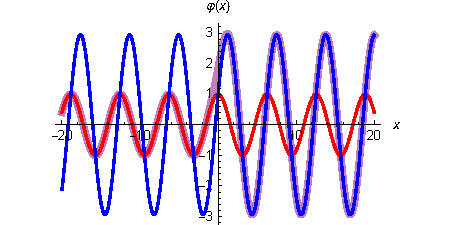
\includegraphics[width=0.4\textwidth]{figures/w3.pdf}
    \caption{Изменение амплитуды и фазы синса в w3, №5 }
    \label{fig:w3}
\end{figure}

На \ref{fig:w3} явно видно, как невозмущенный синус (красная линяя) переходит в возмущенный синус (синяя линяя), в итоге и получается наше решение (фиолетовая линия). 



